% CEE C181/C281 mid-report. Build from this folder: latexmk -pdf mid_report.tex
% Figures: uv run python scripts/mid_report_figures.py (from the repository root), which reads
% the recorded tables in data/ and, for the PeMS panels, data/interim/pems/. Commands for the
% tables behind them: README, "Reproduce the mid-report". The team number and the repository
% link are set in submission.tex.
\documentclass[11pt,letterpaper]{article}
\usepackage[margin=1in]{geometry}
\usepackage[T1]{fontenc}
\usepackage{newtxtext,newtxmath} % Times
\usepackage{graphicx,booktabs,amsmath,tabularx,enumitem}
\usepackage[labelfont=bf]{caption}
\usepackage{float}
\usepackage{placeins} % \FloatBarrier keeps figures inside their subsection
\usepackage{cite} % IEEE numeric citations
\usepackage{microtype}
\usepackage[hidelinks]{hyperref}
\graphicspath{{fig/}}
% Keep figures and tables next to the text that discusses them.
\renewcommand{\topfraction}{0.92}
\renewcommand{\bottomfraction}{0.92}
\renewcommand{\textfraction}{0.06}
\renewcommand{\floatpagefraction}{0.85}
\setcounter{topnumber}{3}
\setcounter{bottomnumber}{2}
\setcounter{totalnumber}{5}
\setlength{\textfloatsep}{10pt plus 2pt minus 2pt}
\setlength{\intextsep}{8pt plus 2pt minus 2pt}
\setlength{\parskip}{4pt}
\setlength{\parindent}{0pt}
\setlist{nosep,leftmargin=1.4em}
\renewcommand{\arraystretch}{1.12}
\newcolumntype{Y}{>{\raggedright\arraybackslash}X}
% The two values to fill in before submission. Rebuild with: latexmk -pdf mid_report.tex
\newcommand{\teamnumber}{[team number]}
\newcommand{\repourl}{[GitHub link to be added: the repository is not published yet]}

\newcommand{\ntests}{135} % automated tests in tests/ (uv run pytest)
\newcommand{\vehh}{\,veh/h}
\newcommand{\ci}[3]{$#1$ [$#2$, $#3$]} % mean [95 % interval]

\begin{document}
\begin{center}
{\Large\bfseries Ramp Metering at the I-405 Southbound Ventura Boulevard On-Ramp:\\[2pt]
The Rules in Use Against a Calibrated ALINEA\par}
\vspace{4pt}
{\large Mid-Report\par}
\vspace{6pt}
Team \teamnumber\par
Manuel A. Martinez Garcia, CEE C281\par
November 19, 2026
\end{center}

\section{Introduction}

The southbound I-405 on-ramp from Ventura Boulevard, at Sepulveda Boulevard in Sherman
Oaks, Los Angeles, is a metered loop ramp. Three lanes queue at the meter, narrow to two
and then to one, and join the freeway over an 85~m acceleration lane
(Figure~\ref{fig:site}). About 25 vehicles fit between the street and the meter. On
Tuesday 11~October 2022 the PeMS mainline station beside the ramp \cite{pems} is below
20~m/s from 06:05 until the end of the study window at 10:00.

I built a microscopic simulation of this ramp and its merge, calibrated its
car-following parameters on PeMS data and checked them on days that were not used, and
ran the metering rules that Caltrans operates \cite{tom2025} against ALINEA
\cite{papageorgiou1991} on the observed morning.

\begin{figure}[!htb]
\centering
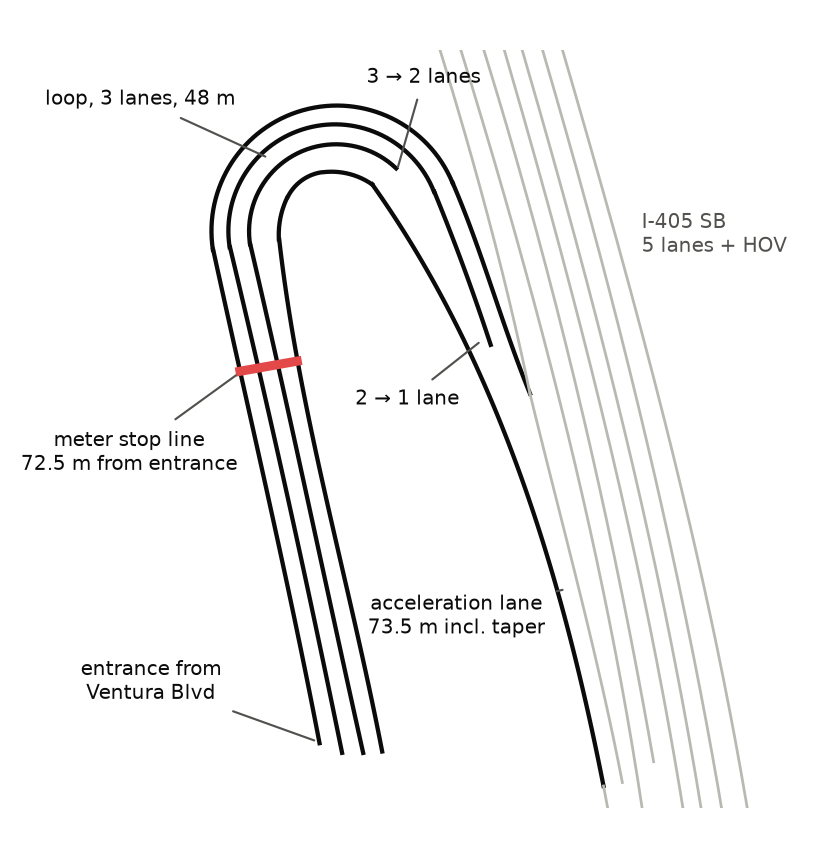
\includegraphics[height=2.7in]{site_geometry.png}\hfill
\raisebox{0.7in}{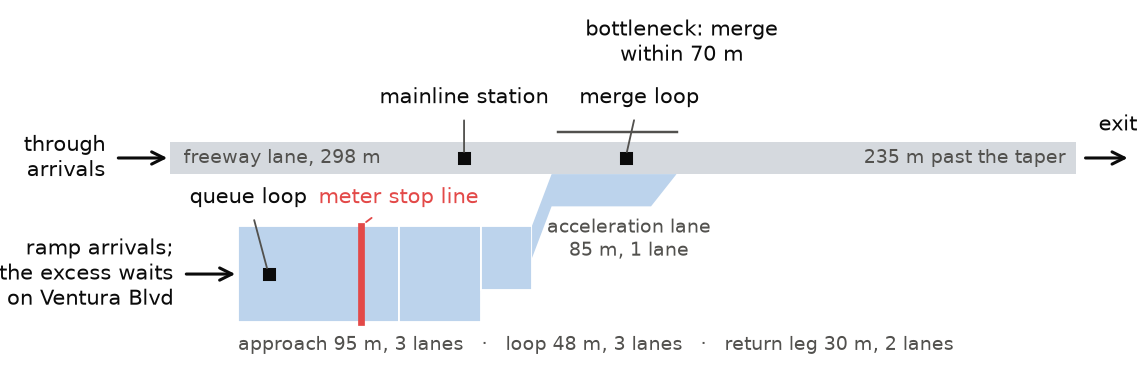
\includegraphics[width=0.57\textwidth]{design_schematic.png}}
\caption{Left: plan view of the ramp measured from the AutoCAD sketch; the red line is
the meter. Right: the simulated segment with its arrivals, exit, bottleneck, meter and
detector loops.}
\label{fig:site}
\end{figure}

\textbf{Question.} \emph{On the observed morning, does a fixed metering rate, the
Caltrans local traffic-responsive plan or ALINEA change persistent congestion beside
this ramp by at least 5~minutes, compared with no meter and with each other? Does the
answer hold when one condition is changed at a time: the demand, how people drive, the
detector, or a rule's own setting?}

\textbf{Definitions.} These make the question testable.
\begin{itemize}
\item \emph{Congested interval:} a 30~s detector interval is congested when its mean
  speed is below 20~m/s (45~mph), or its occupancy is above 15.8~\%.
\item \emph{Persistent congestion:} congestion is persistent when it lasts for at least
  10 consecutive intervals (5~minutes, one PeMS interval). Anything shorter is a
  disturbance. The primary measure is the number of minutes of persistent congestion.
\item \emph{Where and when:} the mainline loop 51.5~m upstream of the gore; Tuesday
  11~October 2022, 05:00--10:00.
\item \emph{A difference counts} when the 95~\% $t$ interval of the differences, paired
  over 10 random seeds, excludes zero and its mean is at least 5~minutes.
\item \emph{Secondary measures:} the time in the system per vehicle that asked to enter,
  with all waiting outside the segment included, and the largest number of vehicles held
  on Ventura Boulevard.
\end{itemize}
The speed threshold is the line that separates the two branches of the PeMS data. The
occupancy threshold is the occupancy at which the calibrated model's lane reaches
capacity (Section~\ref{sec:idm}).

\textbf{Traffic mechanisms behind the question.} A driver keeps a gap $s$ that grows
with speed $v$, about $s_0+vT$. The gap fixes the time headway $h=(s+L)/v$ for vehicle
length $L$, and with it the flow $q=1/h$ and the density $k=1/(s+L)$, so that $q=kv$.
Flow has a maximum, the capacity, because beyond it closer following no longer makes up
for lower speed. At the merge, ramp and through traffic share one lane. When their sum
exceeds what the lane passes, a queue grows at the rate demand minus capacity. A merging
vehicle also makes its follower brake. With spare gap the disturbance dies out; near
capacity it travels upstream and the merge then discharges less than before. A meter
holds ramp vehicles so that the merge stays at its critical occupancy. It should
therefore matter only near capacity, and only while the vehicles it holds fit on the
ramp. Two facts about this site work against it. The ramp stores about 25 vehicles, and
in the peak the merge sits inside a queue that reaches it from farther downstream
(Section~\ref{sec:site}).

\textbf{Predictions.} Eight predictions were written into the repository before the
study ran and were not edited afterwards (Table~\ref{tab:pred}). The three that carry the
question are these. (P1)~At the observed demand no rule makes a counted difference,
because the merge is inside a queue for most of the morning. (P2)~ALINEA's reduction
counts in at least one of three unsaturated cases (10~\% less demand, 25~\% less ramp
demand, a free exit) and in none of four saturated ones. (P3)~Where ALINEA and the
Caltrans plan differ by a counted amount, ALINEA has less congestion, because it reads
the merge and the plan reads a station upstream of it.

\textbf{Status of the evidence.} The PeMS values in this report are observed. Every
simulated value comes from a model that is calibrated only in part and driven by one
observed day. The simulated results are candidates for discussion, not findings about
the site.

\textbf{Repository.} \repourl

\section{Model and parameters}

\subsection{Vehicle motion: the Intelligent Driver Model}\label{sec:idm}

Vehicles follow the Intelligent Driver Model (IDM) of Treiber et al.\ \cite{treiber2000}.
Vehicle $i$ has two states, the position of its front bumper $x_i$ (m) and its speed
$v_i$ (m/s). Its inputs come from the leader $i-1$: the net gap $s_i=x_{i-1}-x_i-L$ and
the closing speed $\Delta v_i=v_i-v_{i-1}$. The model is
\begin{align}
\dot x_i &= v_i, \label{eq:state}\\
\dot v_i &= a\left[1-\left(\frac{v_i}{v_0}\right)^{\delta}
  -\left(\frac{s^*(v_i,\Delta v_i)}{s_i}\right)^{2}\right], \label{eq:idm}\\
s^*(v,\Delta v) &= s_0+\max\!\left(0,\;vT+\frac{v\,\Delta v}{2\sqrt{ab}}\right).
  \label{eq:sstar}
\end{align}
The first term in the bracket is the free-road acceleration; it fades as the vehicle
nears its desired speed $v_0$. The second term is the interaction: braking grows as the
gap $s_i$ falls toward the desired gap $s^*$. The desired gap grows with speed through
the time gap $T$, and closing on the leader ($\Delta v>0$) enlarges it, so braking
starts earlier. Equations~\eqref{eq:idm} and~\eqref{eq:sstar} are Eqs.~6 and~7 of
\cite{treiber2000} with its second jam distance set to zero, as in its Table~I, and with
the lower bound on the dynamic part used in the author's notes \cite{treiberIDM}.
Setting $\dot v_i=0$ and $\Delta v_i=0$ gives the equilibrium gap, flow and density,
\begin{equation}
s_e(v)=\frac{s_0+vT}{\sqrt{1-(v/v_0)^{\delta}}},\qquad
q_e(v)=\frac{v}{L+s_e(v)},\qquad k_e(v)=\frac{1}{L+s_e(v)},
\label{eq:eq}
\end{equation}
which is the model's fundamental diagram. Its maximum is the static capacity $q_c$, at
the speed $v_c$ and density $k_c=q_c/v_c$. A loop of length $\ell$ is covered by each
vehicle over $L+\ell$, so the critical occupancy is
\begin{equation}
o_c=k_c\,(L+\ell).
\label{eq:occ}
\end{equation}
With the values of Table~\ref{tab:idm}, $q_c=1{,}980$\vehh{} per lane at
$v_c=23.8$~m/s: a time headway of 1.82~s, a density of 23.1~veh/km and, for the 1.83~m
loop, an occupancy of 15.8~\%. Motion is integrated with a constant-acceleration step of
$h=0.5$~s, $v^{n+1}=v^n+h\dot v^n$ and $x^{n+1}=x^n+hv^n+\tfrac12h^2\dot v^n$, which
stops a vehicle exactly when its speed would cross zero.

\begin{table}[!htb]
\centering
\caption{Parameters of vehicle motion. ``Paper'' is Table~I of \cite{treiber2000};
``realistic'' is the range given in the author's notes \cite{treiberIDM}. The
calibration is described in Section~\ref{sec:calmethod} and its result in
Section~\ref{sec:cal}.}
\label{tab:idm}
\begin{tabularx}{\textwidth}{l>{\hsize=.75\hsize}Y>{\hsize=.75\hsize}Y>{\hsize=.9\hsize}Y>{\hsize=1.6\hsize}Y}
\toprule
 & Meaning & Value used & Paper; realistic & How the value was set\\
\midrule
$v_0$ & desired speed & 29.1~m/s freeway & 33.3~m/s; --- & calibrated: free-flow branch of the PeMS fundamental diagram, 10--12 Oct 2022\\
 & & 11, 7, 12~m/s ramp & & assumed for the approach, the loop and the return leg\\
$T$ & time gap & 1.51~s & 1.6~s; 0.8--2~s & calibrated: $q_c$ equals the largest observed flow, 1{,}978\vehh{} per lane\\
$\delta$ & acceleration exponent & 20 & 4; --- & calibrated: shape of the free-flow branch\\
$a$ & acceleration & 2.5~m/s$^2$ & 0.73; 0.8--2.5~m/s$^2$ & chosen among 1.5, 2.0 and 2.5 by the ramp vehicles served on three days\\
$b$ & comfortable braking & 2.0~m/s$^2$ & 1.67; about 2~m/s$^2$ & sourced; loop data cannot identify it\\
$s_0$ & standstill gap & 2~m & 2~m; --- & sourced; no standstill is observed\\
$L$ & vehicle length & 5~m & 5~m; --- & paper\\
$b_\text{safe}$ & lane-change safety limit & 4.0~m/s$^2$ & --- & assumed\\
$b_\text{max}$ & braking limit & 8.8~m/s$^2$ & --- & about 0.9~$g$ on dry pavement, assumed\\
\bottomrule
\end{tabularx}
\end{table}

\textbf{Curves and braking.} IDM has no curvature term, so the loop enters the model
through $v_0$ alone: 7~m/s, assumed from a radius of about 15~m. Drivers anticipate a
slower section. With $x_j$ the start of a downstream section and $v_{0,j}$ its desired
speed,
\begin{equation}
v_0(x)=\min\Bigl(v_{0,\text{here}},\;\min_{x_j>x}\sqrt{v_{0,j}^2+2b\,(x_j-x)}\Bigr),
\label{eq:anticipate}
\end{equation}
the highest speed from which the curve speed can be reached braking at the comfortable
$b$. IDM has no braking limit either, so the acceleration is bounded below by
$-b_\text{max}$. The model has no lateral motion, lane width or sight distance.

\textbf{Lane changes and merging.} Only mandatory lane changes are modeled. A vehicle
whose lane ends within 70~m moves to the adjacent lane when the safety criterion of
MOBIL \cite{kesting2007} holds: the IDM acceleration of its new follower, and its own
behind its new leader, must both be at least $-b_\text{safe}$, with both gaps positive.
Yielding is a project rule, not taken from a source: inside the merge zone a freeway
vehicle treats the nearest ramp vehicle ahead of it as its leader when it can follow it
with a deceleration of at most $b_\text{safe}$.

\textbf{Driver variation.} Each vehicle can carry its own $a$, $b$, $T$, $s_0$,
$b_\text{safe}$ and a factor on $v_0$. For a parameter with fixed value $\bar\theta$ and
spread $c_\theta$, driver $i$ has
\begin{equation}
\theta_i=\bar\theta\,\phi_i,\qquad \mathrm{E}[\phi_i]=1,\qquad
\mathrm{sd}[\phi_i]=c_\theta,
\label{eq:driver}
\end{equation}
with $\phi_i$ drawn from a truncated normal or a lognormal distribution, from a random
stream separate from the arrivals. The baseline uses $c_\theta=0$, identical drivers.
Two cases of the study use spreads taken from other sites and other models.

\subsection{Simulated segment}

The segment (Figure~\ref{fig:site}, Table~\ref{tab:geom}) is the smallest one that
contains arrivals, an exit, a bottleneck and a controlled ramp-entry queue. It has one
freeway lane, the lane next to the ramp. Lengths were measured from an AutoCAD sketch of
the ramp. Each run covers 18{,}000~s (05:00--10:00).

\begin{table}[!htb]
\centering
\caption{Geometry of the simulated segment. Desired speeds on the ramp are assumed.}
\label{tab:geom}
\begin{tabularx}{\textwidth}{l>{\hsize=.85\hsize}Y>{\hsize=1.15\hsize}Y}
\toprule
Element & Value & Basis\\
\midrule
Ramp approach & 3 lanes, 95~m, 11~m/s & sketch\\
Ramp loop & 3 lanes, 48~m, 7~m/s & sketch (middle-lane arc)\\
Ramp return leg & 2 lanes, 30~m, 12~m/s & sketch\\
Acceleration lane & 1 lane, 85~m, 29.1~m/s & sketch (11.5~m to the gore, then 73.5~m of lane and taper)\\
Freeway lane & 298~m to the taper end, 235~m beyond & sketch (traced edge lengths)\\
Meter stop line & 72.5~m from the ramp entrance & sketch (red line)\\
Storage before the meter & 24.6 vehicles & $3\times72.5$~m at 8.84~m per vehicle \cite{rmdm2022}\\
Merge zone & last 70~m of the acceleration lane & assumed\\
\bottomrule
\end{tabularx}
\end{table}

\subsection{Boundary conditions and demand}\label{sec:boundary}

\textbf{Arrivals.} Ramp and through vehicles arrive as Poisson processes. Their rates
follow the 5-minute counts of the PeMS on-ramp station (716744) and of the five-lane
mainline station (717816) \cite{pems}, held constant over 60~s. The engine has one
freeway lane, so two assumptions map the five-lane station onto it. The first is lane
balance: with station flow $q_\text{ML}$ and ramp flow $q_\text{R}$,
\begin{equation}
q_\text{lane}=\frac{q_\text{ML}+q_\text{R}}{5},\qquad
q_\text{thru}=q_\text{lane}-q_\text{R},
\label{eq:balance}
\end{equation}
where $q_\text{lane}$ is the flow the modeled lane carries past the merge and
$q_\text{thru}$ its through traffic. On the observed day the ramp asks for 48 to
1{,}116\vehh{} (3{,}380 vehicles in all) and the through traffic for 197 to
1{,}853\vehh{} (3{,}449 vehicles); their sum peaks at 2{,}009\vehh{} at 05:40
(Figure~\ref{fig:inputs}). A vehicle that finds no room at an entrance waits in a
boundary queue, which for the ramp is Ventura Boulevard. Its wait is counted and it is
never dropped. The demand builder refuses a window that contains a missing or
PeMS-imputed interval.

\textbf{Exit.} The second assumption is the downstream boundary. The freeway lane ends
235~m past the taper. While the PeMS station speed is at least 20~m/s the outflow is
free. Otherwise the exit passes the observed flow: the last vehicle out continues as a
virtual leader at the speed $v_b$ on the congested branch that satisfies
\begin{equation}
q_e(v_b)=q_\text{lane},\qquad v_b<v_c ,
\label{eq:exit}
\end{equation}
in Eq.~\eqref{eq:eq}. On the observed day the exit is limited in 235 of the 300 minutes,
with $v_b$ between 3.1 and 15.3~m/s. This boundary keeps its observed values in every
case except the one that removes it. It encodes what the station data show: in the peak
the queue at the merge comes from downstream (Section~\ref{sec:site}). Two consequences
matter for the results. Once the freeway is congested, observed flow is a lower bound
on demand, so the observed day sits at about capacity by construction. And a vehicle
held at the meter leaves part of the exit's allowance unused.

\begin{figure}[!htb]
\centering
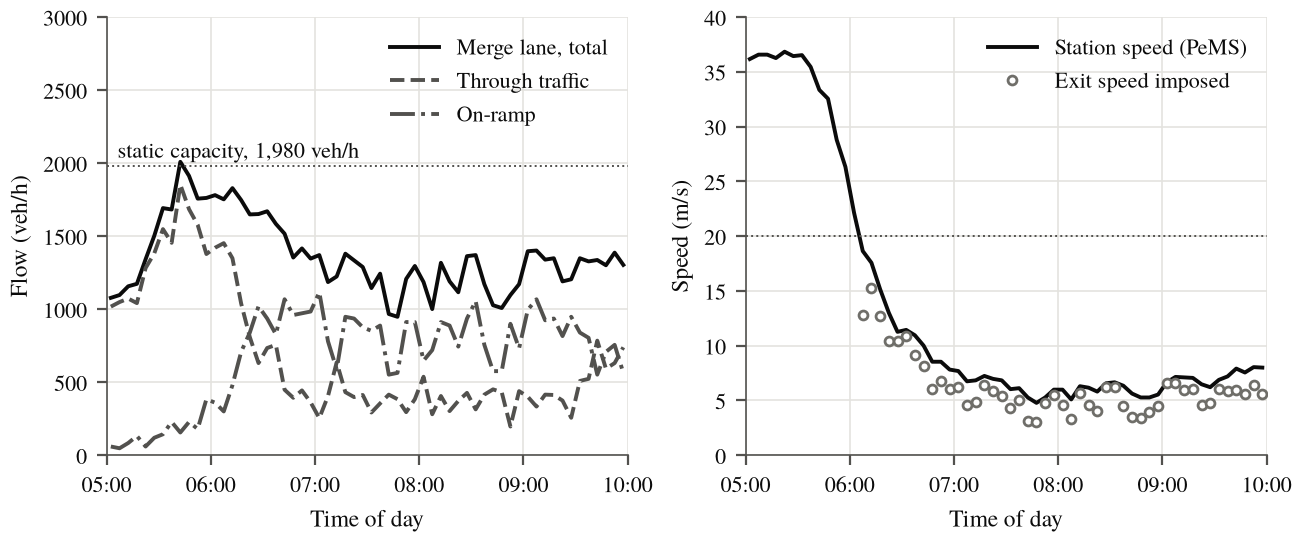
\includegraphics[width=0.92\textwidth]{inputs.png}
\caption{Inputs on the observed day. Left: observed ramp flow, the merge-lane flow of
Eq.~\eqref{eq:balance} and its through traffic, with the static capacity of the
calibrated model. Right: observed station speed and the exit speed $v_b$ of
Eq.~\eqref{eq:exit} imposed in congested intervals.}
\label{fig:inputs}
\end{figure}

\subsection{Detectors and what the controller knows}\label{sec:detectors}

All rules use loop records only: 1.83~m loops that report a count, an occupancy (the
share of the interval in which the loop is covered) and a mean speed every 30~s. There
are four loops: the mainline station 51.5~m upstream of the gore, which the Caltrans
plan reads and where congestion is measured; a loop in the merge area, 43.5~m past the
gore, which ALINEA reads; a queue loop 18~m from the ramp entrance; and a passage loop
just past the stop line. With cumulative counts $N$, the controller's estimates of the
ramp queue and of the next interval's ramp demand are
\begin{equation}
\hat n_t=N^\text{queue loop}_t-N^\text{passage}_t,\qquad
\hat d_t=\frac{N^\text{queue loop}_t-N^\text{queue loop}_{t-1}}{\Delta t},\qquad
\Delta t=30~\text{s}.
\label{eq:estimate}
\end{equation}
The estimate $\hat n_t$ cannot exceed what fits between the two loops, in practice the
$3\times54.5$~m of lane between the queue loop and the stop line, and it does not see
the vehicles still on the street.

\subsection{Metering rules}\label{sec:control}

Four rules are compared. Each releases one vehicle per green. The ramp is listed with
two metered lanes \cite{rmdp2017,rmdp2023}; the three lanes at the stop line share that
two-lane rate, alternating. Rates are bounded to 240--900\vehh{} per lane
\cite{rmdm2022}, that is $r_\text{min}=480$ and $r_\text{max}=1{,}800$\vehh{}.

\emph{No meter} and a \emph{fixed rate} of 8~veh/min per lane (960\vehh{}) are the
baselines.

\emph{Caltrans local traffic-responsive metering} is the method normally in place in
District~7 \cite{d7report2014,topd2112,tom2025}. Every 30~s the occupancy $o_t$ of the
mainline station selects one of $N=15$ plan levels, and a rate for $n=2$ lanes,
\begin{equation}
\ell_t=\min\!\left(N-1,\;\max\!\left(0,\left\lfloor
\frac{o_t-o_1}{o_N-o_1}(N-1)\right\rfloor\right)\right),\qquad
r^\text{plan}_t=n\left[\rho_1+\ell_t\,\frac{\rho_N-\rho_1}{N-1}\right],
\label{eq:plan}
\end{equation}
with thresholds $(o_1,o_N)=(0.05,\,0.20)$ and rates $(\rho_1,\rho_N)=(900,\,240)$\vehh{}
per lane. A queue override has priority. While the queue loop is covered for at least
half of an interval, the rate steps up from the applied rate,
$r_t=\max(r^\text{plan}_t,r_{t-1})+n\,\Delta\rho$ with $\Delta\rho=120$\vehh{} per lane,
and it returns to the plan in one step when the loop clears.

\emph{ALINEA} \cite{papageorgiou1991} integrates the occupancy error at the merge loop,
\begin{equation}
r^\text{A}_{t}=r_{t-1}+K_R\,(\hat o-o_t),
\label{eq:alinea}
\end{equation}
where $r_{t-1}$ is the rate applied in the last interval, after its bounds. This is
Eq.~14 of \cite{papageorgiou1991} and the form given in the course lecture \cite{ma2026}.
The paper places the set value $\hat o$ at the critical occupancy, so here
$\hat o=o_c=0.158$ from Eq.~\eqref{eq:occ}; this is what ``calibrated ALINEA'' means in
this report. The gain is $K_R=1.5$~veh/s per unit occupancy (54\vehh{} per percentage
point); the paper found 70 adequate and its results insensitive to the value. Queue
control follows ALINEA/Q \cite{smaragdis2003}: the rate that returns the estimated ramp
queue to its target $n^*=20$ vehicles within one interval is applied when it is larger,
\begin{equation}
r^\text{Q}_t=\hat d_t+\frac{\hat n_t-n^*}{\Delta t},\qquad
r_t=\min\bigl(r_\text{max},\,\max(r_\text{min},\,r^\text{A}_t,\,r^\text{Q}_t)\bigr).
\label{eq:alineaq}
\end{equation}
When its detector reports nothing, ALINEA holds the last rate for 60~s and then applies
the fixed rate.

The structure of the Caltrans rule is sourced. Its numbers for this ramp are not
published: the plan thresholds and rates follow a published plan for another ramp
\cite{shladover2017}, and the queue trigger, the fixed rate, the ALINEA gain and the
queue target are assumptions (Table~\ref{tab:control}).

\begin{table}[!htb]
\centering
\caption{Control values and their basis.}
\label{tab:control}
\begin{tabularx}{\textwidth}{>{\hsize=.8\hsize}Y>{\hsize=1.1\hsize}Y>{\hsize=1.1\hsize}Y}
\toprule
Item & Value in the model & Basis\\
\midrule
Update and detector interval & 30~s & Caltrans manual \cite{tom2025}\\
Rate limits & 240--900\vehh{} per lane, 2 lanes & Caltrans design manual \cite{rmdm2022}\\
Plan thresholds and rates & 15 levels, 900 at $\le5$~\% down to 240 at $\ge20$~\% & form: \cite{tom2025}; values: \cite{shladover2017}, assumed for this ramp\\
Queue override step & $+120$\vehh{} per lane per update & Caltrans manual \cite{tom2025}\\
Queue loop position & 18~m from the entrance, 3/4 back from the stop line & Caltrans design manual \cite{rmdm2022}\\
Queue trigger & loop covered $\ge50$~\% of 30~s & assumed\\
Fixed rate & 8~veh/min per lane & District~7 example, assumed here\\
ALINEA set value $\hat o$ & 0.158 & critical occupancy of the calibrated model, as in \cite{papageorgiou1991}\\
ALINEA gain $K_R$ & 1.5~veh/s per unit occupancy & assumed; varied in the study\\
Queue target $n^*$ & 20~veh & assumed: 80~\% of the storage (see Section~\ref{sec:open})\\
\bottomrule
\end{tabularx}
\end{table}

\subsection{Calibration procedure}\label{sec:calmethod}

There is no single standard for calibrating a traffic microsimulation. The nearest is
the FHWA Traffic Analysis Toolbox \cite{fhwa2004,fhwa2019}: check the model for errors
first, adjust as few parameters as possible, calibrate capacity before system
performance, and validate on data that were not used. I followed it in two steps.

\emph{Step 1, the fundamental diagram.} The data are the 5-minute values of station
717816 in intervals where all five lanes are observed: 861 intervals on 10, 11 and
12~October 2022 for calibration and 1{,}429 on five other days held out. Following
Dervisoglu et al.\ \cite{dervisoglu2009}, $v_0$ is the least-squares slope of flow on
density over the points above 55~mph, and the capacity $q^\text{obs}_c$ is the largest
observed flow. For each acceleration exponent on a grid from 4 to 60 the time gap
solves
\begin{equation}
\max_v\,q_e(v;\,v_0,T,\delta)=q^\text{obs}_c ,
\label{eq:capmatch}
\end{equation}
and the smallest $\delta$ whose root-mean-square flow error on the calibration days is
within 5~\% of the best is taken. Loop data identify these three parameters and no
others: $a$ and $b$ do not enter Eq.~\eqref{eq:eq}, and no standstill is observed, so
$s_0$ cannot be fitted. A parameter whose regime is missing from the data should not be
calibrated \cite{treiberkesting2013cal}.

\emph{Step 2, the whole model.} The acceleration $a$ sets what the modeled merge passes
after it has broken down. By a rule written before the run, it is the value among 1.5,
2.0 and 2.5~m/s$^2$ with the smallest mean absolute error in ramp vehicles served on
the three calibration days. That value is then scored on three held-out days against
FHWA's example criteria \cite{fhwa2004}: quantities within 15~\% of the observed value,
and
\begin{equation}
\mathrm{GEH}=\sqrt{\frac{2\,(E-V)^2}{E+V}}<5
\label{eq:geh}
\end{equation}
for simulated and observed hourly flows $E$ and $V$.

\subsection{Study design}\label{sec:design}

The baseline is the calibrated scenario on the observed day. Each of 34 further cases
changes exactly one thing and keeps the rest, the rules' settings included
(Table~\ref{tab:cases}); an automated test checks that every case changes one thing and
that the change takes effect. Every case runs under the four rules with seeds 1 to 10:
$35\times4\times10=1{,}400$ runs of five simulated hours. Within a seed, every rule
meets the same arrivals. Three differences are reported, all paired by seed: each rule
minus no meter, one rule minus another, and each case minus the baseline. Before the
run, the capacity, the deterministic queue and the capping strategy of the course
lectures \cite{ma2026} were computed for every case without simulation
(Section~\ref{sec:formulas}).

\begin{table}[!htb]
\centering
\caption{The 35 cases of the one-factor study. Percentages are relative to the baseline.}
\label{tab:cases}
\begin{tabularx}{\textwidth}{@{}l>{\hsize=1.25\hsize}Y>{\hsize=.75\hsize}Y@{}}
\toprule
Group & What changes, one case each & Cases\\
\midrule
Baseline & nothing & 1\\
Demand & ramp and mainline demand together $\times0.9$, $\times1.1$; ramp demand alone $\times0.75$, $\times1.25$; through traffic alone $\times0.75$, $\times1.25$; through traffic as observed in the lane next to the ramp (an upper bound); demand oscillating by $\pm50$~\% with a period of 10 or 60~min; no downstream restriction (free exit) & 10\\
Car following & $T$ 1.21 and 1.81~s ($\pm20$~\%); $a$ 2.0 and 3.0~m/s$^2$ ($\pm20$~\%); $b$ 1.0 and 3.0~m/s$^2$; $s_0$ 1 and 3~m; $v_0$ on the freeway lane 26.2 and 32.0~m/s ($\pm10$~\%); $\delta=4$ & 11\\
Drivers & $v_0$, $T$, $a$, $b$ drawn per driver with a spread of 11.55~\%; spreads reported at other sites & 2\\
Information & ALINEA's detector reports nothing from 06:30 to 07:30 & 1\\
Rule settings & ALINEA: gain halved, doubled; set value $\pm20$~\%; no queue rule. Caltrans plan: thresholds at 3--12~\% and at 8--32~\% occupancy; no queue override. Fixed rate: 6 and 12~veh/min per lane & 10\\
\bottomrule
\end{tabularx}
\end{table}

\textbf{Checks.} \ntests{} automated tests cover, among other things, vehicle
conservation in every step, the IDM equilibrium gap, the discharge of the exit boundary
(within 3~\%), the plan steps and the override, the curve anticipation and the braking
limit, and that ALINEA's set value equals the critical occupancy of whatever
configuration is loaded. In the 1{,}400 runs every vehicle is accounted for and no step
has overlapping vehicles.

\section{Results so far}

\subsection{The site in the data}\label{sec:site}

Before simulating, I checked whether this merge is the bottleneck. Figure~\ref{fig:pems}
shows the observed day, and Table~\ref{tab:site} the eight October 2022 weekdays on
which station 717816 is fully observed, at lane level and with observed lanes only.

\begin{figure}[!htb]
\centering
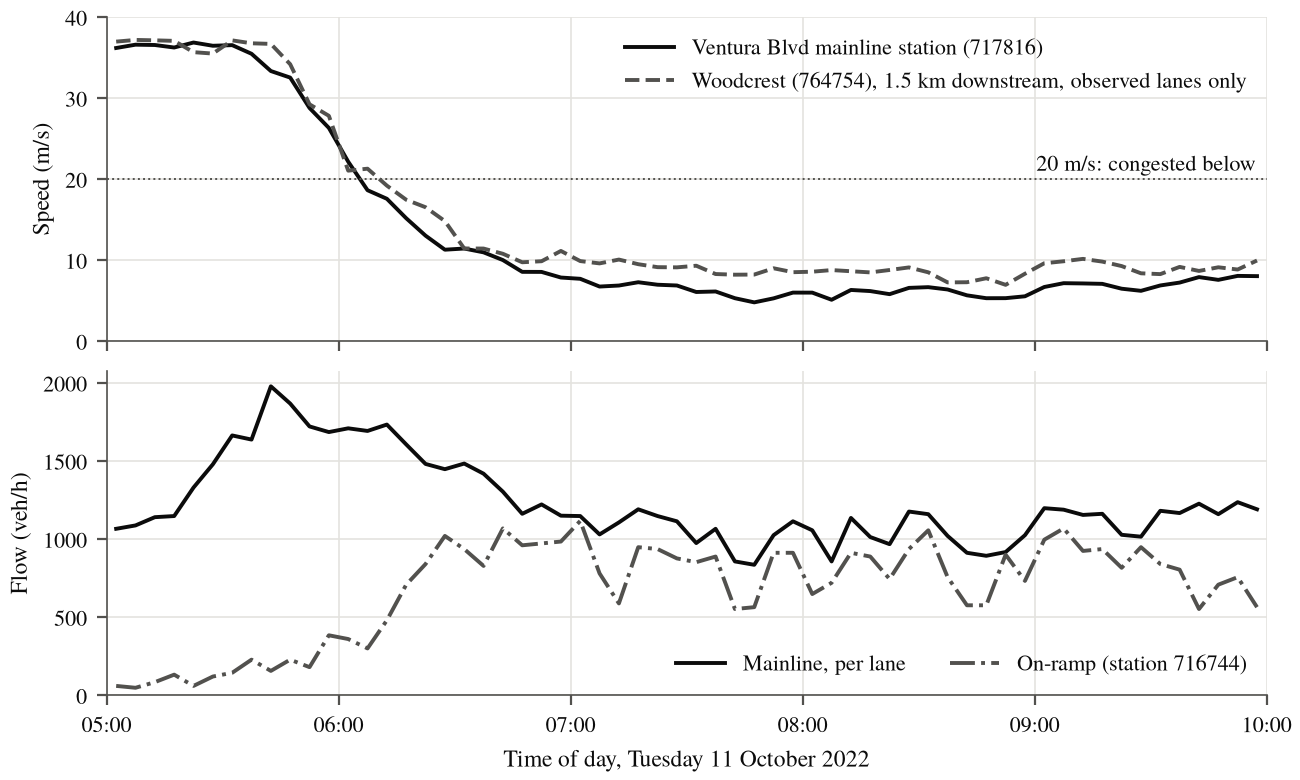
\includegraphics[width=0.9\textwidth]{pems_day.png}
\caption{PeMS 5-minute data, Tuesday 11~October 2022. Top: speed at the mainline station
beside the ramp and at the next observed station downstream, with the 20~m/s line of the
congestion definition. Bottom: flow per lane at the mainline station and flow of the
on-ramp.}
\label{fig:pems}
\end{figure}

\begin{table}[!htb]
\centering
\setlength{\tabcolsep}{4.2pt}
\caption{Observed PeMS data on eight weekdays of October 2022. Onset is the first of
three consecutive 5-minute intervals below 20~m/s. Royal Ridge is 2.4~km downstream of
the ramp. Flows and speeds are means from 07:00 to 08:55.}
\label{tab:site}
\begin{tabular}{lrrrrrrrr}
\toprule
Day of October 2022 & 3 & 10 & 11 & 12 & 14 & 24 & 25 & 28\\
\midrule
Onset at the ramp (Ventura) & 06:00 & 06:10 & 06:05 & 06:00 & 06:10 & 06:00 & 06:05 & 06:20\\
Onset at Royal Ridge & 06:05 & 06:05 & 06:10 & 06:10 & 06:25 & 06:15 & 06:20 & 06:15\\
Mainline flow at the ramp (veh/h) & 4,960 & 5,112 & 5,153 & 5,345 & 5,839 & 5,231 & 5,065 & 6,137\\
Speed at the ramp (m/s) & 5.9 & 6.3 & 6.1 & 6.6 & 7.9 & 6.2 & 5.9 & 9.3\\
Speed at Royal Ridge (m/s) & 11.1 & 12.4 & 12.6 & 13.1 & 12.8 & 12.1 & 13.1 & 13.6\\
On-ramp flow (veh/h) & 751 & 682 & 807 & 889 & 728 & 826 & 821 & 689\\
\bottomrule
\end{tabular}
\end{table}

Three things follow. In the peak, from about 06:30 to 10:00, the merge is inside a
queue: both stations downstream are below 20~m/s on all eight days, and the bottleneck
test of Chen et al.\ \cite{chen2004} (upstream below 40~mph and at least 20~mph slower
than downstream, in 5 of 7 consecutive intervals) is met on none of them. The head of
the queue is at or beyond Royal Ridge and cannot be located, because the next 14~km of
mainline stations report no observed data. At onset the picture is different: the ramp
station drops below 20~m/s before Royal Ridge on 6 of the 8 days, and a queue growing
back at the 6 to 7~m/s given by the shockwave formula $w=\Delta q/\Delta k$ would have
reached Royal Ridge first. So the data do not show the congestion arriving from
downstream, and a breakdown at or near this merge at onset is not excluded. Finally,
the ramp is not shut out: it discharges 680 to 890\vehh{} between 07:00 and 08:55. One
caution on the speeds: at this station PeMS reports flow times a fixed length over
occupancy, not a measured speed.

\FloatBarrier
\subsection{Calibration and validation}\label{sec:cal}

\begin{figure}[!htb]
\centering
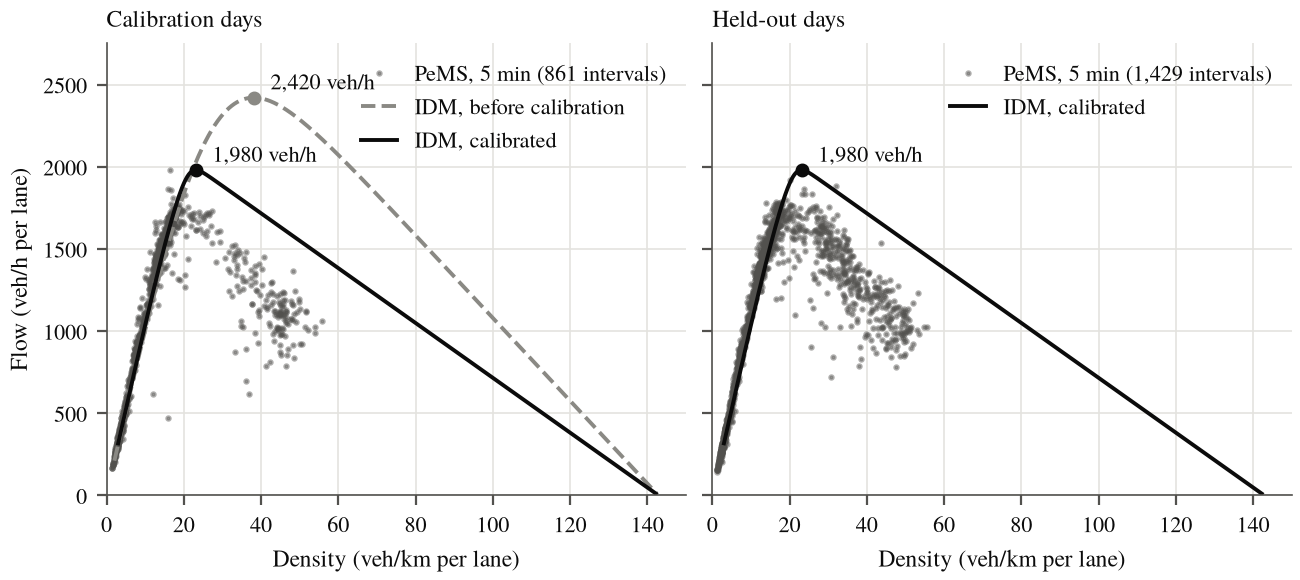
\includegraphics[width=\textwidth]{fd_calibration.png}
\caption{Fundamental diagram of station 717816 (PeMS, 5-minute values) and the IDM
equilibrium curve of Eq.~\eqref{eq:eq}. Left: the three calibration days with the curve
before and after calibration. Right: the five held-out days with the calibrated curve.}
\label{fig:fd}
\end{figure}

Step~1 gives $v_0=29.1$~m/s, $T=1.51$~s and $\delta=20$ (Figure~\ref{fig:fd}). The
exponent matters more than I expected. With the textbook $\delta=4$ the model reaches
capacity at 17~m/s, below the 20~m/s congestion line, while the observed speed at the
twenty highest flows is 27.0~m/s; with $\delta=20$ capacity is reached at 23.8~m/s.
Table~\ref{tab:cal} compares the curve with the observed flow at each observed density.
Over all intervals the error falls from 530 to 256\vehh{} on the calibration days and
from 558 to 271 on the held-out days, and the free-flow branch meets the 15~\% criterion
on the held-out days (87~\% of intervals).
The congested branch does not: 11~\%. The model still gives about 470\vehh{} too much
flow at a congested density, and one equilibrium curve cannot pass through both the
observed capacity and the observed congested states.

\begin{table}[!htb]
\centering
\caption{Flow given by the equilibrium curve at each observed density against the
observed flow: root-mean-square error in veh/h per lane, and the share of intervals
within 15~\%.}
\label{tab:cal}
\begin{tabular}{llrrrrr}
\toprule
 & & Capacity & \multicolumn{2}{c}{Error (veh/h)} & \multicolumn{2}{c}{Within 15~\%}\\
Days & Parameters ($v_0$, $T$, $\delta$) & (veh/h) & free & congested & free & congested\\
\midrule
Calibration & before: 28.6~m/s, 1.0~s, 4 & 2,420 & 111 & 1,086 & 91~\% & 6~\%\\
 & calibrated: 29.1~m/s, 1.51~s, 20 & 1,980 & 88 & 509 & 90~\% & 9~\%\\
Held out & before & 2,420 & 122 & 1,004 & 82~\% & 6~\%\\
 & calibrated & 1,980 & 97 & 472 & 87~\% & 11~\%\\
\bottomrule
\end{tabular}
\end{table}

Step~2 ran the whole model on six days with the Caltrans rule, five seeds each (90
runs). The acceleration $a=2.5$~m/s$^2$ has the smallest error in ramp vehicles served
on the calibration days: 3.2~\%, against 8.2~\% for 2.0 and 22.5~\% for 1.5. On the
three held-out days it meets every criterion (Figure~\ref{fig:val}): vehicles through
the merge lane within 3~\% of the observed count (GEH 0.6 to 1.1), ramp vehicles within
5~\% (GEH 0.2 to 1.3) and congested minutes within 10~\%. On 11~October, the day
used in the study, the model passes 6{,}648 of the 6{,}829 vehicles observed, and its
station is congested for 214~minutes against 235 observed. Two cautions. The value 2.5 is the upper end of the
range tried, and the model still passes slightly fewer vehicles than were observed on
five of the six days, which points at the merge rule more than at how hard drivers
accelerate.

\begin{figure}[!htb]
\centering
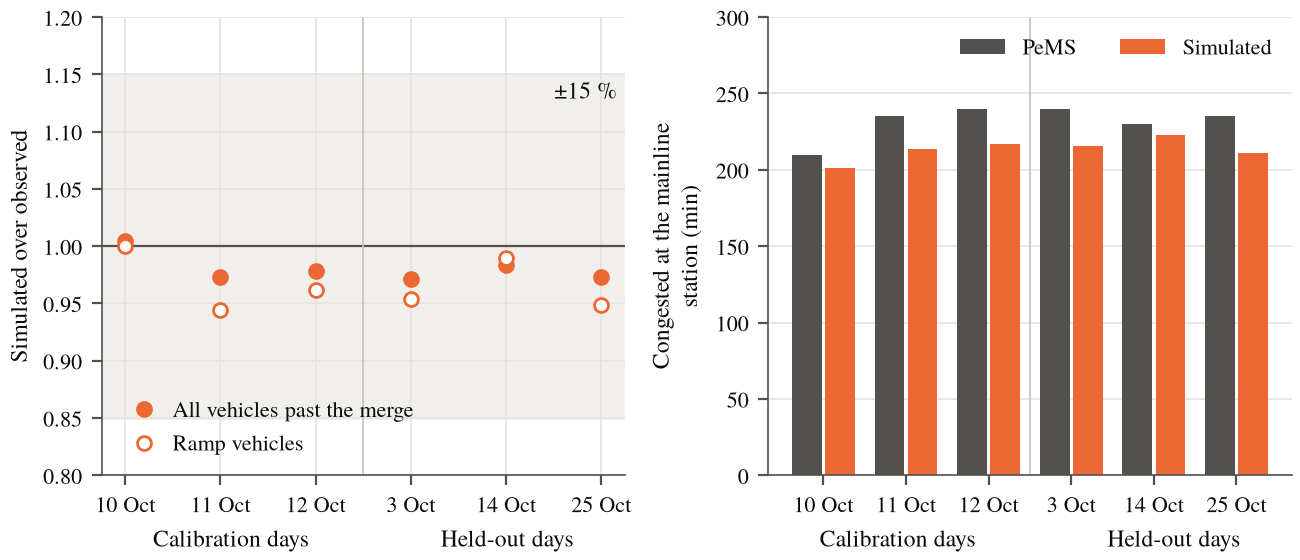
\includegraphics[width=0.9\textwidth]{validation.png}
\caption{The calibrated model ($a=2.5$~m/s$^2$) against PeMS on three calibration days
and three held-out days, means of five seeds. Left: simulated over observed vehicles,
with the 15~\% band of the FHWA example criteria. Right: minutes below 20~m/s at the
mainline station, simulated against observed.}
\label{fig:val}
\end{figure}

\FloatBarrier
\subsection{What the lecture formulas give before any run}\label{sec:formulas}

Table~\ref{tab:formulas} uses 5-minute steps and no simulation. Capacity is the static
capacity $q_c$. The deterministic (D/D/1) queue serves the exit's allowance where the
exit is limited and $q_c$ elsewhere. The last column is how long the capping strategy
of the lecture, $q_\text{ramp}=\max(0,\,q_c-q_\text{in})$, can hold vehicles before the
24.6 vehicles of storage are full and it has to be discontinued \cite{ma2026}.

\begin{table}[!htb]
\centering
\setlength{\tabcolsep}{4pt}
\caption{Course formulas applied to selected cases, without simulation.}
\label{tab:formulas}
\begin{tabular}{lrrrrr}
\toprule
 & Capacity & Peak demand & 5-min intervals & D/D/1 unserved & Minutes the\\
Case & (veh/h) & (veh/h) & above capacity & at 10:00 (veh) & cap can hold\\
\midrule
Baseline & 1,980 & 2,009 & 1 & 0 & 7\\
Demand $\times0.9$ & 1,980 & 1,808 & 0 & 0 & 0\\
Demand $\times1.1$ & 1,980 & 2,210 & 3 & 537 & 10\\
Ramp demand $\times1.25$ & 1,980 & 2,048 & 1 & 800 & 25\\
Through traffic $\times1.25$ & 1,980 & 2,472 & 10 & 615 & 14\\
$T=1.21$~s & 2,375 & 2,009 & 0 & 0 & 0\\
$T=1.81$~s & 1,697 & 2,009 & 8 & 81 & 8\\
\bottomrule
\end{tabular}
\end{table}

At the baseline the formulas leave no queue at 10:00, and the cap could hold vehicles
for 7 of the 300 minutes. Whatever queue the simulation leaves at the baseline is the
cost of the merge, and the room for a meter is small before any run is made.

\FloatBarrier
\subsection{The observed day under the four rules}

At the baseline the four rules are hard to tell apart (Figure~\ref{fig:baseline}). Each
serves 97.1~\% of the vehicles that asked to enter. Time in the system is 6.8 to
7.0~minutes per vehicle, the peak queue on Ventura Boulevard is 148 to 162 vehicles, and
the mainline station is congested for 204 to 214~minutes (means of 10 seeds).

The traces of seed~1 show why. Between 06:05 and 06:45 the exit's allowance is
1{,}520 to 1{,}830\vehh{}, but whenever both approaches are queued the modeled merge
passes only 1{,}440\vehh{}, one ramp vehicle for each through vehicle, 27~\% below the
static capacity. In those periods the merge limits the flow, not the exit boundary,
and the ramp's share is 720\vehh{}. From 06:45 the exit is the limit and the ramp
gets through at about the rate it arrives, 807\vehh{} on average between 07:00 and
08:55. The fixed rate of 960\vehh{} is above both, so it holds almost nothing back.
ALINEA and the Caltrans plan do cut their rates to the minimum of 480\vehh{} at 06:00,
but the plan's override takes over at 06:19 and ALINEA's queue rule at 06:26. Over the
10 seeds ALINEA's queue rule, Eq.~\eqref{eq:alineaq}, set the rate in 464 of the 600
intervals, and the plan's override in 441. With 25 vehicles of storage, the queue on the
ramp decides the rate for three quarters of the morning, not the state of the freeway.
The flat stretch of ALINEA's speed between 06:24 and 06:48 is the one-for-one discharge;
with identical drivers it repeats exactly.

The simulated station is congested for about as long as the real one, but it is not as
slow: about 12~m/s between 07:00 and 09:50 against 5 to 8~m/s in PeMS. This is the
congested branch that the calibration could not fit, together with lane balance, which
leaves the modeled lane about 400\vehh{} of through traffic upstream of the merge where
each real lane carries about 1{,}000. In free flow PeMS reports about 36~m/s before
05:40, above the model's single desired speed of 29.1~m/s.

\begin{figure}[!htb]
\centering
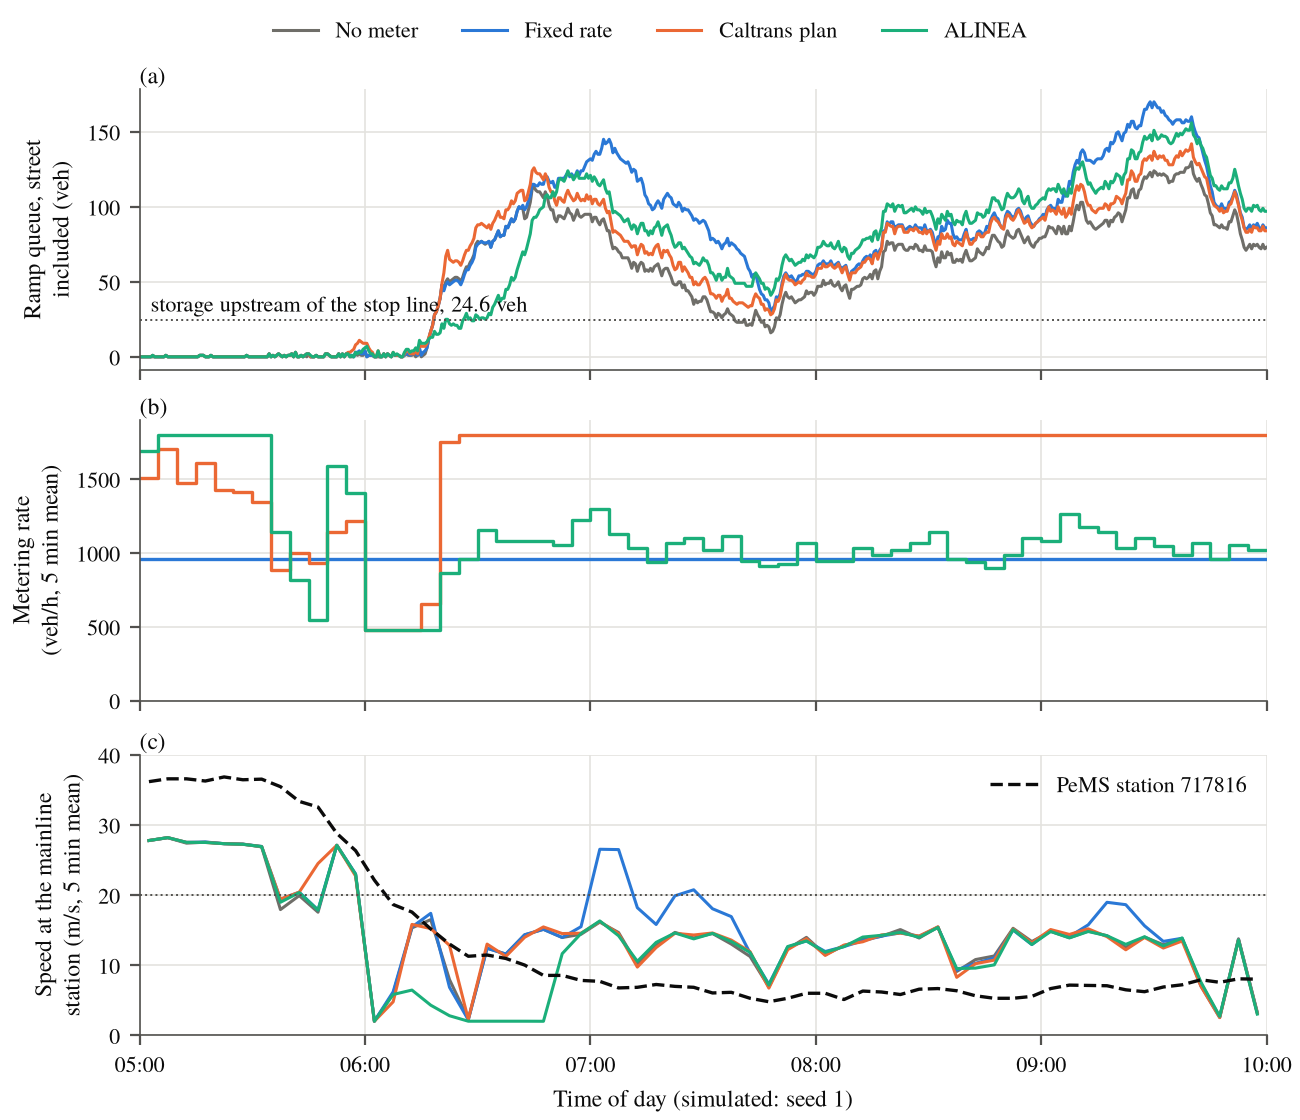
\includegraphics[width=0.86\textwidth]{baseline_day.png}
\caption{The calibrated baseline on the observed day, seed~1. Top: vehicles waiting to
enter from the ramp side, including those held on Ventura Boulevard, with the storage
upstream of the meter. Middle: metering rate. Bottom: speed at the simulated mainline
station against PeMS (mean of the station's five lanes), with the 20~m/s line.}
\label{fig:baseline}
\end{figure}

\FloatBarrier
\subsection{One factor at a time}\label{sec:ablation}

Figure~\ref{fig:rules} shows every rule against no meter in the 25 cases that change
the world, not a rule. Table~\ref{tab:pred} scores the eight predictions.

\begin{figure}[!htb]
\centering
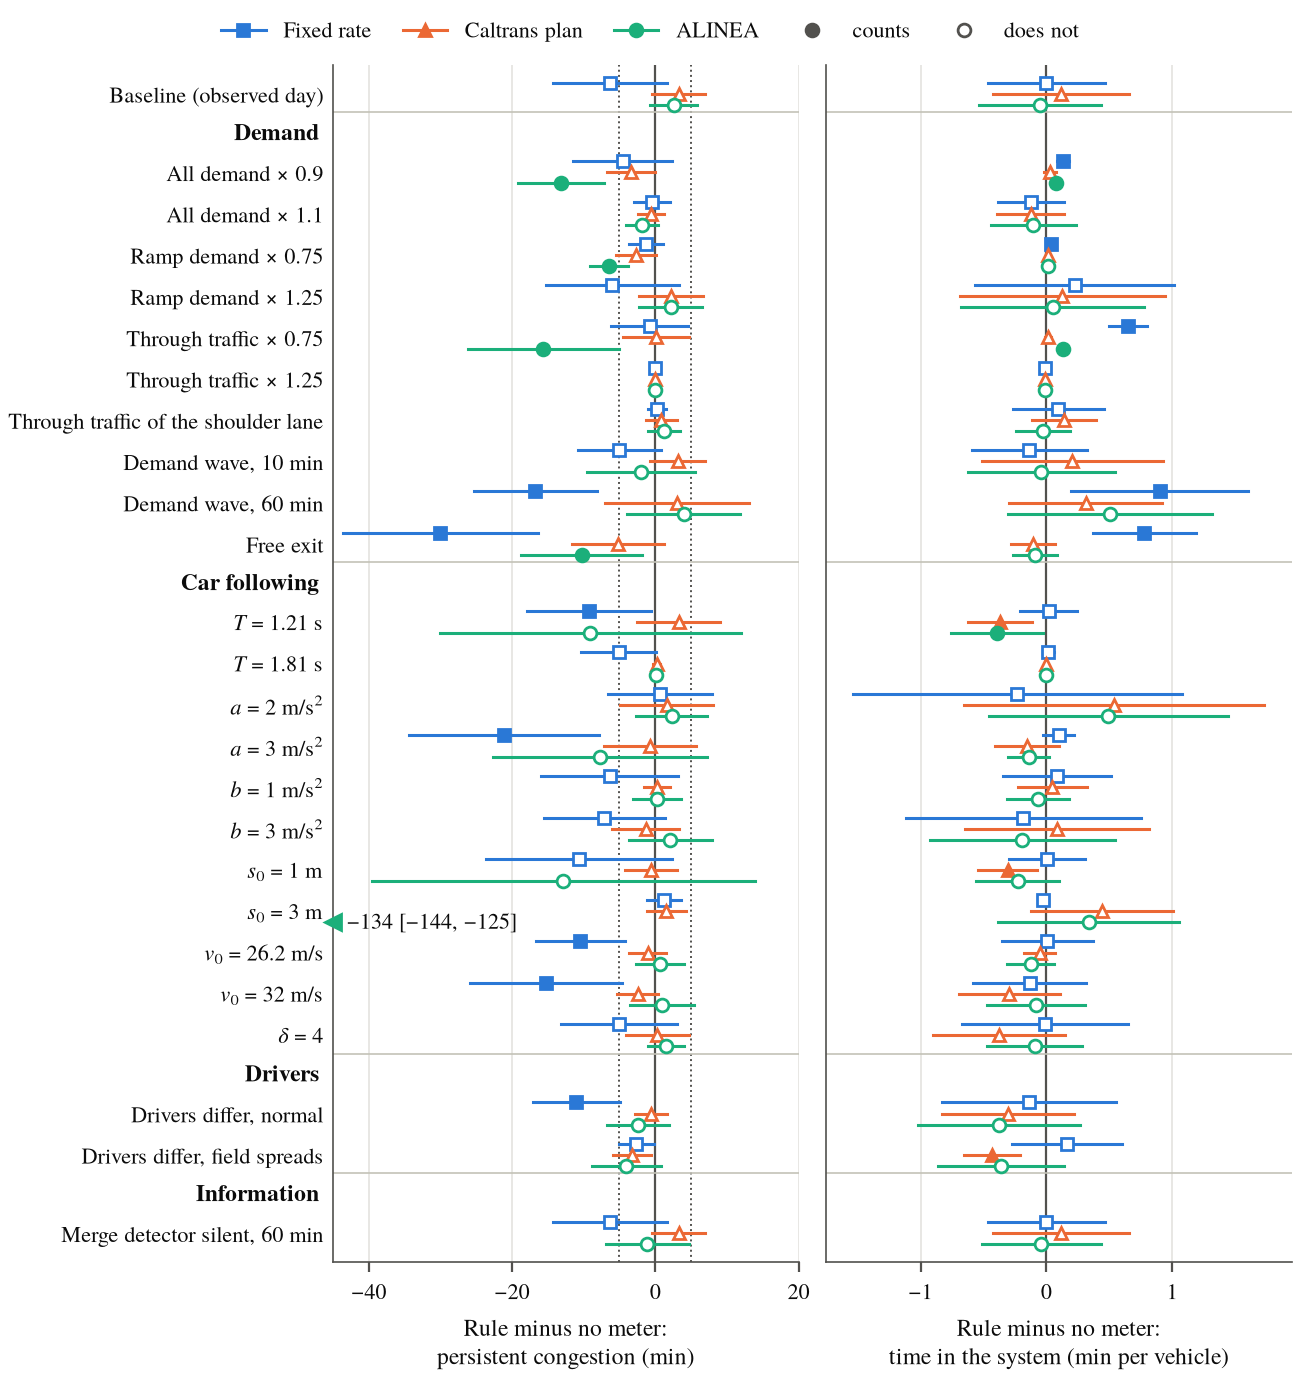
\includegraphics[width=0.94\textwidth]{rule_effects.png}
\caption{Each rule minus no meter in the 25 cases that do not change a rule's setting:
means of 10 seeds, paired, with 95~\% $t$ intervals. Left: minutes of persistent
congestion; a filled marker is a difference that counts (interval excludes zero and
mean of at least 5~minutes). Right: time in the system per vehicle; filled when the
interval excludes zero.}
\label{fig:rules}
\end{figure}

\begin{table}[!htb]
\centering
\small
\caption{The eight predictions, written before the run, and what the 1{,}400 runs
gave. Differences are in minutes of persistent congestion unless stated, as mean and
95~\% interval.}\label{tab:pred}
\begin{tabularx}{\textwidth}{@{}r>{\hsize=.72\hsize}Y>{\hsize=.38\hsize}Y>{\hsize=1.9\hsize}Y@{}}
\toprule
 & Prediction & Outcome & Evidence\\
\midrule
1 & At the baseline no rule makes a counted difference & Contradicted & Against no meter none counts: fixed \ci{-6.3}{-14.3}{+1.6}, plan \ci{+3.2}{-0.5}{+7.0}, ALINEA \ci{+2.5}{-0.7}{+5.8}. But the fixed rate has less congestion than ALINEA by \ci{8.9}{1.0}{16.8} and than the plan by \ci{9.6}{2.3}{16.9}\\
2 & ALINEA helps where the merge is not saturated, and only there & Supported & Counts with 10~\% less demand \ci{-13.2}{-19.1}{-7.2}, 25~\% less ramp demand \ci{-6.5}{-9.2}{-3.8} and a free exit \ci{-10.2}{-18.7}{-1.8}; in none of the four saturated cases (means $-1.9$ to $+2.1$)\\
3 & Where ALINEA and the plan differ by a counted amount, ALINEA has less congestion & Supported & Five counted differences, all for ALINEA, among them 10~\% less demand \ci{-9.8}{-16.1}{-3.4} and 25~\% less through traffic \ci{-15.7}{-24.8}{-6.6}. None for the plan\\
4 & How people drive moves the outcome more than any rule: $T$ by more than 20 congested minutes, $a$ by more than 1~min per vehicle & Contradicted for $T$, supported for $a$ & From $T=1.21$ to 1.81~s without a meter: \ci{-9.9}{-21.8}{+2.0} congested minutes, but \ci{+10.5}{+10.0}{+11.1}~min per vehicle. From $a=2.0$ to 3.0~m/s$^2$: \ci{-7.5}{-8.7}{-6.3}~min per vehicle. The largest effect of a rule at the baseline is 0.12~min per vehicle\\
5 & ALINEA is insensitive to its gain and set value & Supported & ALINEA against itself at the baseline: gain halved \ci{0.0}{-3.0}{+3.0}, doubled \ci{+1.2}{-0.8}{+3.3}; set value $-20$~\% \ci{+1.1}{-1.3}{+3.5}, $+20$~\% \ci{+1.0}{-0.3}{+2.3}\\
6 & The queue rule and the override are what take the meter out of play & Supported for ALINEA, contradicted for the plan & ALINEA without its queue rule: \ci{-174.3}{-179.9}{-168.7} and \ci{+128}{+109}{+146} vehicles on the street. The plan without its override: \ci{-4.8}{-8.2}{-1.5}, below the 5-minute line, and \ci{+2}{-19}{+22} vehicles\\
7 & With its detector missing, ALINEA behaves as the fixed rate & Supported & Every ALINEA run falls back in 118 of the 120 intervals of the fault; ALINEA minus fixed is \ci{+5.2}{-2.5}{+13.0}\\
8 & Drivers that differ do not reorder the rules, and they add delay & Supported & No rule contrast counts with the opposite sign; with the field spreads, time per vehicle without a meter rises by \ci{4.2}{3.4}{5.1}~min\\
\bottomrule
\end{tabularx}
\end{table}

\textbf{What the rules do.} At the observed demand no rule differs from no meter, which
is what P1 expected. P1 is still contradicted, because the rules differ from each
other: the fixed rate has about 9 fewer congested minutes than either responsive rule.
That is not a gain. The fixed rate is the only rule
that never gives way to the ramp queue, so it holds more vehicles on the street. In no case is its
time per vehicle lower than without a meter by more than the interval allows, and in
five cases it is higher. The
same trade shows when a rule is allowed to hold (Figure~\ref{fig:trade}). ALINEA
without its queue rule removes 172 of the 211 congested minutes, holds 127 more vehicles
on Ventura Boulevard and costs 1.7~minutes more per vehicle. A fixed rate of 6~veh/min
per lane removes 136 congested minutes, holds 336 more vehicles and costs 4.7~minutes
more per vehicle. Part of this cost comes from the downstream boundary, which passes a
set flow in congested intervals whether or not the ramp uses it.

\begin{figure}[!htb]
\centering
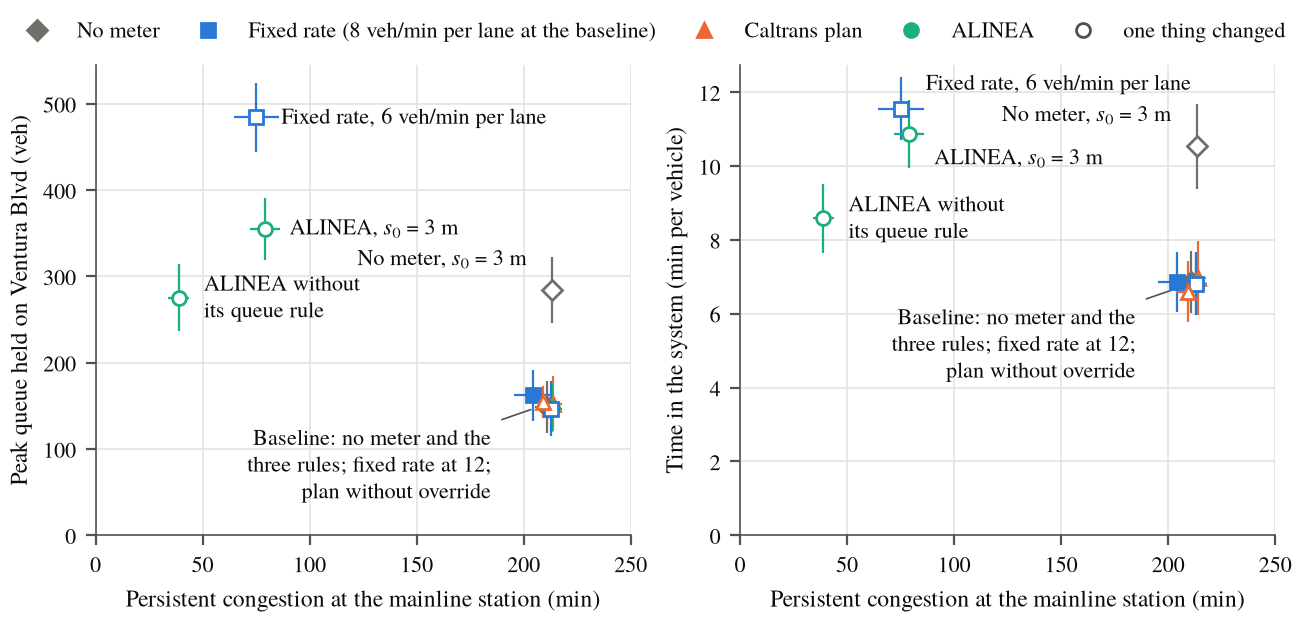
\includegraphics[width=0.92\textwidth]{tradeoff.png}
\caption{Freeway congestion against the cost of holding vehicles, means of 10 seeds with
95~\% intervals: the four rules at the baseline (filled), and runs in which one setting or parameter
was changed (hollow). Left: peak queue on Ventura Boulevard. Right: time in the system
per vehicle.}
\label{fig:trade}
\end{figure}

Below saturation the meter does help the freeway. ALINEA cuts congestion by 13~minutes
with 10~\% less demand, by 7 with 25~\% less ramp demand, by 16 with 25~\% less through
traffic and by 10 with a free exit; the Caltrans plan makes a counted difference in
none of the 25 cases. Even there, time per vehicle is not lower with ALINEA (it changes
by $-0.09$ to $+0.13$~minutes). In this model the meter moves the wait from the freeway
lane to the ramp. It does not remove it.

\textbf{What the world does.} Figure~\ref{fig:cases} puts these effects next to what
one changed condition does without any meter. A 20~\% longer time gap adds
8.4~minutes per vehicle, 20~\% less acceleration adds 5.8, and drivers that differ as
reported at other sites add 4.2. Ten per cent more demand adds 10.8~minutes per
vehicle and 541 vehicles to the street queue. The largest effect of any rule at the
baseline is 0.12~minutes. The acceleration $a$, which loop data cannot identify, moves
time per vehicle from 5.2 to 12.7~minutes across the range tried. How well the
car-following model is calibrated matters more here than which rule runs.

\begin{figure}[!htb]
\centering
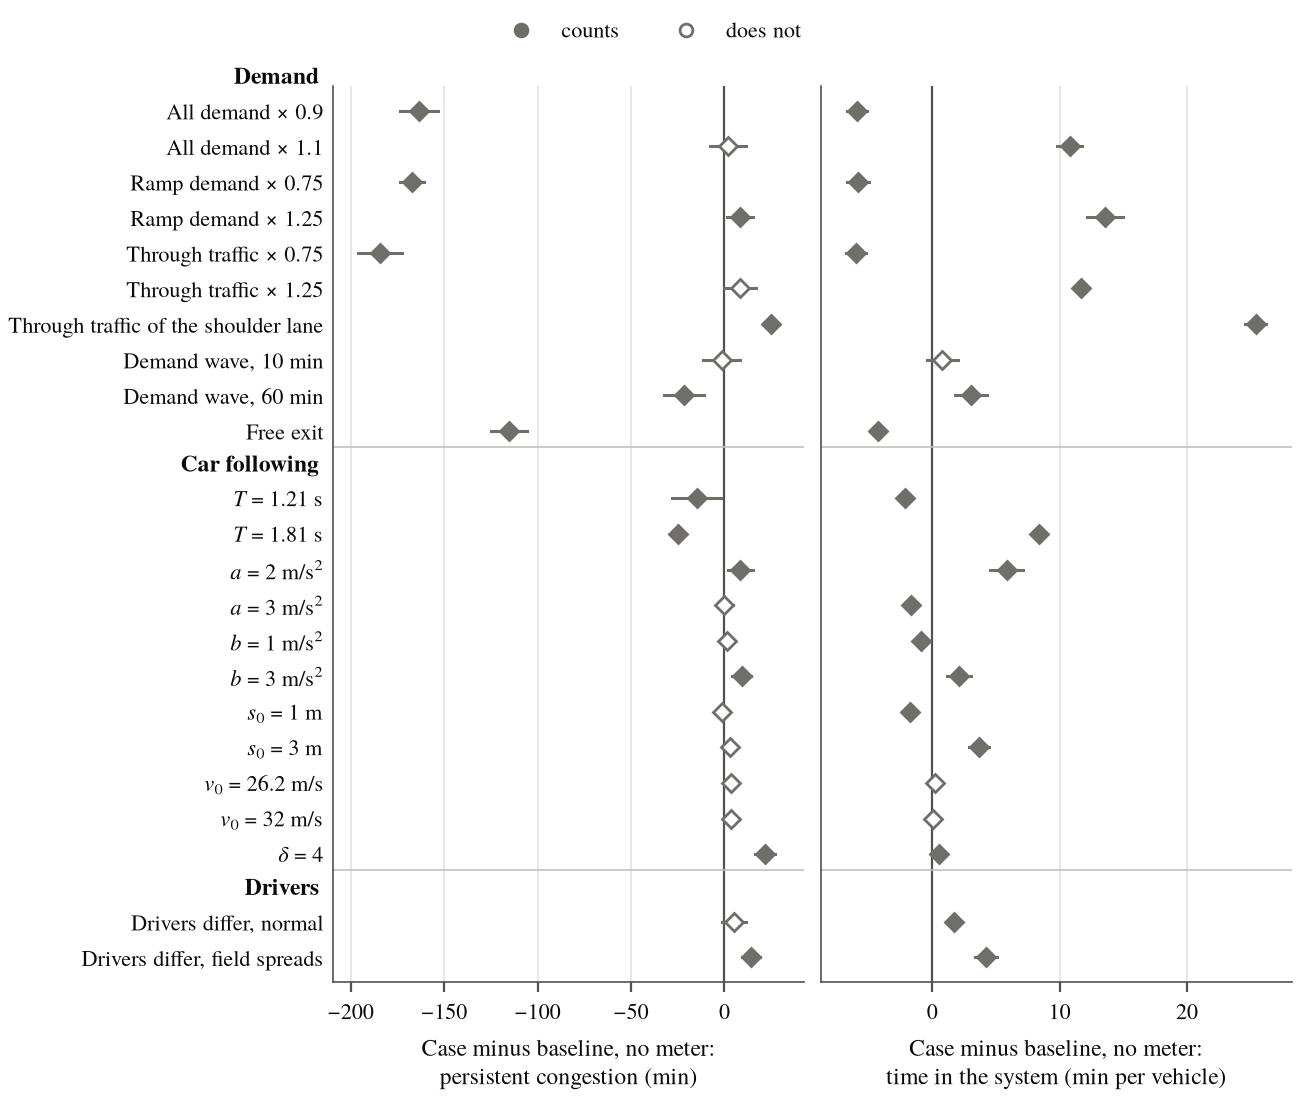
\includegraphics[width=0.8\textwidth]{case_effects.png}
\caption{Each case minus the baseline, without a meter: means of 10 seeds, paired, with
95~\% $t$ intervals. Left: minutes of persistent congestion. Right: time in the system
per vehicle.}
\label{fig:cases}
\end{figure}

\textbf{Two things the run exposed.} First, with a standstill gap of 3~m ALINEA cut
congestion by 134~minutes and held 71 more vehicles on the street, as if it had no queue
rule. A check after the run (seed~1) shows why: at 8~m per queued vehicle only 20.4
vehicles fit between the queue loop and the stop line, so the estimate $\hat n$ of
Eq.~\eqref{eq:estimate} stays at the target $n^*=20$ while 238 vehicles wait on average. The queue rule works at the baseline
only because 23.4 vehicles fit at 7~m. Second, minutes of congestion saturate. With
$T=1.81$~s the station records fewer congested minutes than the baseline (186 against
211) while time per vehicle more than doubles, because vehicles that cannot enter the
modeled lane wait outside it. This is why P4 failed for $T$, and above saturation time
per vehicle is the measure to trust.

\FloatBarrier
\subsection{Trajectories}

Figure~\ref{fig:traj} shows a case where ALINEA counts, 10~\% less demand, for the seed
whose difference is closest to the mean (seed~4) and the half hour in which the two runs
differ most. Without a meter the queue from the merge covers the freeway lane upstream
of the gore until about 06:21. With ALINEA it has cleared by 06:17. Over the half hour
the mean speed upstream of the gore is 10.4~m/s without a meter and 16.0~m/s with
ALINEA.

\begin{figure}[!htb]
\centering
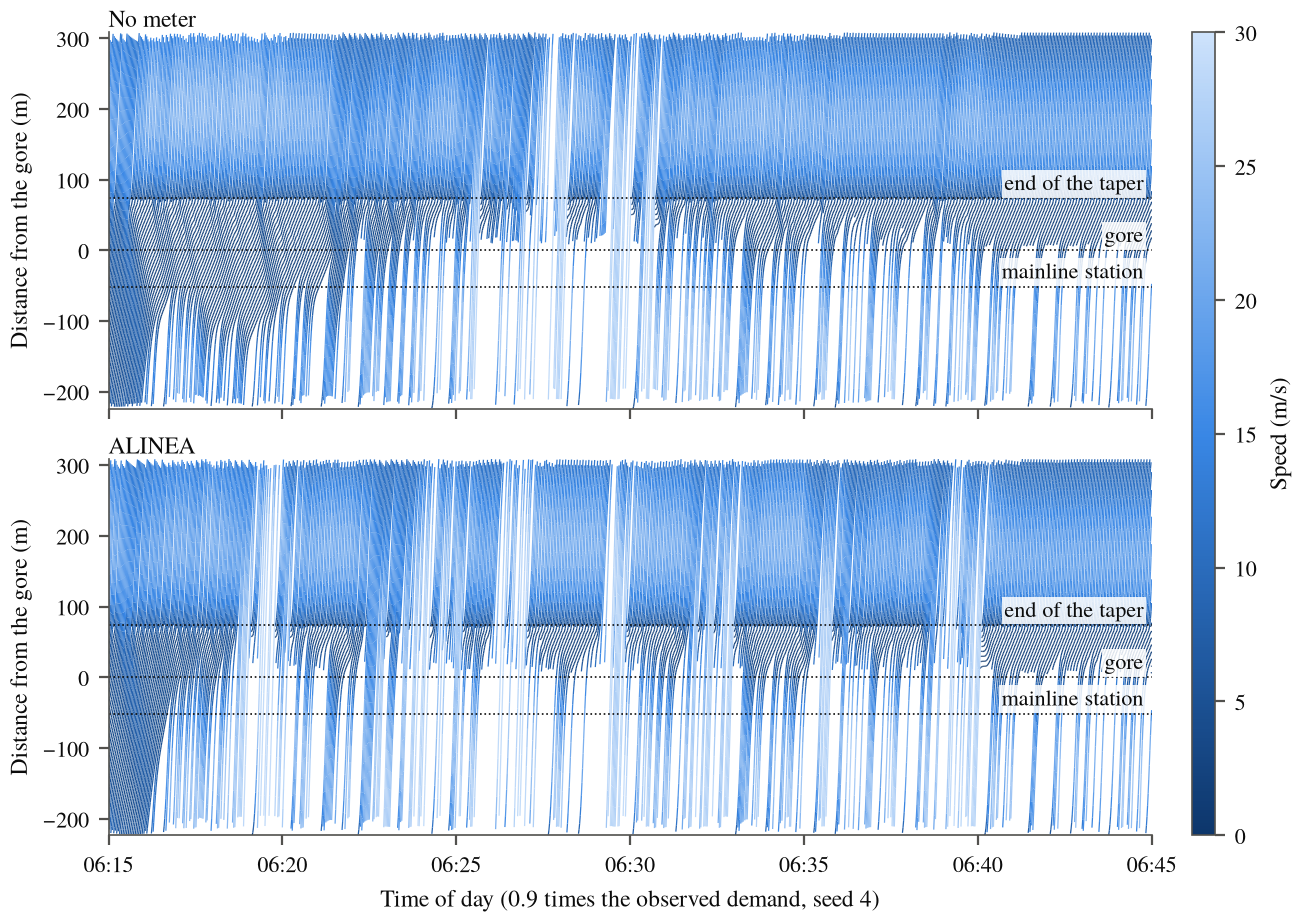
\includegraphics[width=0.9\textwidth]{timespace.png}
\caption{Trajectories on the freeway lane with 10~\% less demand, seed~4, 06:15 to
06:45, colored by speed. Top: no meter. Bottom: ALINEA. Horizontal lines mark the
mainline station ($-51.5$~m), the gore and the end of the taper ($+73.5$~m).}
\label{fig:traj}
\end{figure}

\FloatBarrier
\subsection{Ramp demand against mainline demand}

An earlier study of 960 runs, on the model before calibration, scaled ramp demand and
through traffic separately (Figure~\ref{fig:mix}). It answered the idea this project
started from, that a congested mainline keeps ramp traffic out. Raising through traffic
by 25~\% lowered ramp exits by 536 vehicles (505 to 567), close to the 492 through
vehicles added while the exit is limited: below about half of the merge's output, each
added mainline vehicle takes one ramp vehicle's place. With the through traffic observed
in the lane next to the ramp, both approaches are queued and they share: the ramp keeps
2{,}561 exits and 1{,}461 mainline vehicles are left unserved, in line with the
turn-taking reported at congested merges \cite{cassidy2005,bargera2010}. No rule
changed the ramp's exits by 2~\% or more in any of 36 comparisons. Four of that study's
five predictions were supported; the fifth, that more ramp demand buys the ramp nothing
at the upper bound, failed narrowly (2.5~\% against a line of 2~\%).

\begin{figure}[!htb]
\centering
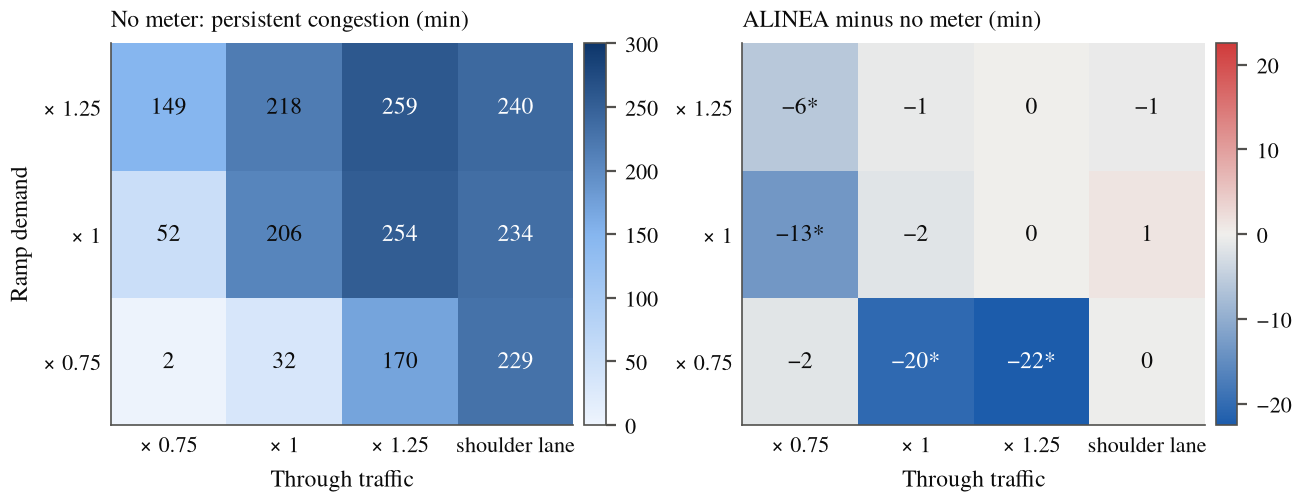
\includegraphics[width=0.9\textwidth]{mix_study.png}
\caption{Ramp demand against through traffic, flow-limited exit, model before
calibration, means of 10 seeds. Left: minutes of persistent congestion without a meter.
Right: ALINEA minus no meter in the same cells; an asterisk marks a difference that
counts.}
\label{fig:mix}
\end{figure}

\FloatBarrier
\subsection{What the controller knows}

The course asks for a state estimate and a short forecast scored against a simple
baseline. I scored the two the meter already uses, Eq.~\eqref{eq:estimate}, on the
baseline day (ALINEA, seed~1, from 06:00). The last-value forecast of the next 30~s of
ramp arrivals has a mean absolute error of 1.20 vehicles per interval, against 1.30 for
a ten-interval moving average; with the queue loop missing for an hour both rise to
about 2.0. The queue estimate is within 1.8 vehicles while the queue fits upstream of
the stop line, which is 11~\% of the time. Over all samples it is short by 63 vehicles,
because it cannot see past the queue loop.

\FloatBarrier
\section{Challenges}

\subsection{Resolved}
\begin{itemize}
\item \emph{The model was not calibrated, and one time gap could not fit both capacity
  and congestion.} I followed the FHWA procedure: three parameters from the fundamental
  diagram, one from system performance, and a check on held-out days
  (Section~\ref{sec:cal}). The free-flow branch and the flows through the merge now meet
  the example criteria. The congested branch does not, and that part stays open below.
\item \emph{ALINEA's set value was wrong.} It stood at 34~\%, eight points above the
  critical occupancy of the model at the time. The rule was checked against the 1991
  paper and the lecture, $\hat o$ was set to the critical occupancy, and a test now
  recomputes it for every configuration. A test of 30 runs then found no counted
  difference between the two values, against the prediction written before it.
\item \emph{Was the merge the bottleneck at all?} The station-level check of the first
  draft said the congestion came from downstream. The lane-level check with the
  bottleneck test of \cite{chen2004} supports that for the peak but not for the onset
  (Section~\ref{sec:site}), and it found that one upstream station reports a speed that
  contradicts its own flow and occupancy.
\item \emph{A five-lane station had to drive a one-lane model.} Lane balance,
  Eq.~\eqref{eq:balance}, with a flow-matched exit, Eq.~\eqref{eq:exit}, is tested to
  within 3~\%. The lane next to the ramp as observed gives an upper bound, used as a
  case.
\item \emph{Three seeds and one day.} Comparisons now use 10 seeds with paired
  intervals and a stated size, and the validation uses six days.
\item \emph{Impossible braking and overlapping vehicles.} IDM braked at up to
  15.4~m/s$^2$ entering the loop. Drivers now anticipate it,
  Eq.~\eqref{eq:anticipate}, and braking is bounded. The 1{,}400 runs record no
  overlap.
\item \emph{The team changed.} The project became an individual one and forecasting was
  dropped. The repository was cleaned around one question, with one run command.
\end{itemize}

\subsection{Open, with the plan}\label{sec:open}
\begin{itemize}
\item \emph{The course's final pathway.} The guide requires a CAV or a traffic-signal
  controller on the supplied scaffold in addition to ramp metering. I have not started
  it. Plan: confirm with the instructor what it is for an individual project, obtain the
  scaffold, and build a baseline and one controller with one stress test.
\item \emph{The queue rule depends on what its loops can count.} The target of 20
  vehicles was set from the whole storage, but the loops can count 23.4 vehicles at the
  model's 7~m per vehicle and only 18.5 at the 8.84~m of the Caltrans manual. Plan: set
  the target as a share of the countable storage, add the queue loop's occupancy as a
  second trigger, and rerun the cases this touches.
\item \emph{The congested branch and the merge.} The model gives too much flow at a
  congested density, and $a$ sits at the top of its range. With both approaches queued
  the merge passes 1{,}440\vehh{}, 27~\% below the static capacity, and while the
  freeway lane flows near capacity no ramp vehicle gets in at all: none between 06:10
  and 06:20 in seed~1 without a meter, where PeMS shows 480 and then 708\vehh{} entering.
  A yielding driver also ignores the leader in its own lane. Plan: let the yielding driver take the lower of the two IDM
  accelerations, then repeat the validation on the six days; the change is kept only if
  the held-out criteria are still met.
\item \emph{Minutes of congestion saturate.} Plan: report time per vehicle and the
  street queue next to it everywhere, and add delay by origin (ramp or mainline).
\item \emph{One freeway lane and an imposed exit.} All the benefit of a held ramp
  vehicle goes to one lane, and the exit's allowance does not react to the meter. The
  head of the queue cannot be located in the data. Plan: state it as a limit, and bound
  it with the free-exit case and a case with the allowance changed by $\pm10$~\%.
\item \emph{Unknowns about the site.} This ramp's plan table, a possible HOV bypass
  lane and the loop positions are assumed. Plan: a count on site on 20~November (how
  the meter runs, the queue on the ramp and the street, where the mainline station
  sits), and a request to Caltrans District~7.
\item \emph{One observed day and many comparisons.} Each measure has 105 comparisons of
  a rule with no meter, so a counted difference in a single case is a candidate. Plan:
  repeat the baseline and the cases that count on a second day (14~October) and with
  seeds 11 to 20.
\item \emph{A source I could not read.} The queue rule follows \cite{smaragdis2003} as
  described in secondary sources; I could not open the paper. Plan: obtain it through
  the library and check Eq.~\eqref{eq:alineaq} against it.
\end{itemize}

\section{Timeline}\label{sec:timeline}

Table~\ref{tab:timeline} lists the tasks up to the final paper. For each test the
expected outcome is stated now, so that the result can contradict it. The plan is
feasible because the whole study reruns from one command in about two hours on this
machine, and the validation in about ten minutes.

\begin{table}[H]
\centering
\caption{Dated tasks up to the final paper.}\label{tab:timeline}
\begin{tabularx}{\textwidth}{@{}l>{\hsize=.93\hsize}Y>{\hsize=1.07\hsize}Y@{}}
\toprule
Date (2026) & Task & Prediction stated now, or deliverable\\
\midrule
Thu 19 Nov & Submit this report; publish the repository & ---\\
Fri 20 Nov & Count on site, 07:15: meter cycle, queue on the ramp and the street, station position. Confirm the final pathway with the instructor & the queue passes the entrance during the peak; the meter releases one vehicle per green in two lanes\\
Sat 21 Nov & Tie the queue target to the countable storage; rerun the rule-setting and standstill-gap cases & ALINEA with $s_0=3$~m no longer differs from no meter by a counted amount\\
Mon 23 Nov & Revise the yield rule; repeat the validation on six days & held-out flows stay within 15~\% and no run records an overlap; $a=2.0$ fits as well as 2.5 does now\\
Tue 24 Nov & Add delay by origin; exit allowance $\pm10$~\% & with 10~\% more allowance ALINEA's reduction counts at the observed demand\\
Wed 25 Nov & Second observed day (14~Oct): baseline and the cases that count, seeds 1--20 & ALINEA's reduction with 10~\% less demand keeps its sign and counts\\
Fri 27 Nov & Final pathway on the course scaffold: baseline and one controller & one comparison and one stress case, with a decision trace\\
Mon 30 Nov & Freeze results; rebuild every figure and table from the repository & one command reproduces the paper's figures\\
Tue 1 Dec & Final paper draft and slides & comparisons, stress tests and the final-pathway part\\
Wed 2 Dec & Final presentation and paper & ---\\
\bottomrule
\end{tabularx}
\end{table}

If ALINEA's gain below saturation fades on the second day, the paper will report a
negative result for this ramp.

\begin{thebibliography}{99}
\setlength{\itemsep}{2pt}

\bibitem{pems}
California Department of Transportation, ``Performance Measurement System (PeMS),
Station 5-Minute data, District~7, October 2022, stations 716744, 717816, 764754 and
717807.'' Accessed: Nov. 2026. [Online]. Available: \url{https://pems.dot.ca.gov}

\bibitem{tom2025}
California Department of Transportation, \emph{Traffic Operations Manual}, ch.~215,
pt.~4, ``Ramp metering operations.'' Sacramento, CA, USA: Caltrans, Apr. 2025.

\bibitem{papageorgiou1991}
M.~Papageorgiou, H.~Hadj-Salem, and J.-M.~Blosseville, ``ALINEA: A local feedback
control law for on-ramp metering,'' \emph{Transp. Res. Rec.}, no.~1320, pp.~59--64,
1991.

\bibitem{treiber2000}
M.~Treiber, A.~Hennecke, and D.~Helbing, ``Congested traffic states in empirical
observations and microscopic simulations,'' \emph{Phys. Rev.~E}, vol.~62, no.~2,
pp.~1805--1824, Aug. 2000, doi: 10.1103/PhysRevE.62.1805.

\bibitem{treiberIDM}
M.~Treiber, ``The Intelligent-Driver Model and its variants.'' Accessed: Nov.~15, 2026.
[Online]. Available: \url{https://traffic-simulation.de/info/info_IDM.html}

\bibitem{kesting2007}
A.~Kesting, M.~Treiber, and D.~Helbing, ``General lane-changing model MOBIL for
car-following models,'' \emph{Transp. Res. Rec.}, vol.~1999, pp.~86--94, 2007,
doi: 10.3141/1999-10.

\bibitem{rmdm2022}
California Department of Transportation, \emph{Ramp Metering Design Manual}.
Sacramento, CA, USA: Caltrans, Oct. 2022.

\bibitem{rmdp2017}
California Department of Transportation, \emph{2017 Ramp Metering Development Plan}.
Sacramento, CA, USA: Caltrans, 2017, p.~110 (LA-405 PM~39.09, southbound Ventura
Boulevard).

\bibitem{rmdp2023}
California Department of Transportation, \emph{2023 Ramp Metering Development Plan}.
Sacramento, CA, USA: Caltrans, 2023, Table~10.

\bibitem{d7report2014}
California Department of Transportation, District~7, \emph{2014 Ramp Metering Annual
Report}. Los Angeles, CA, USA: Caltrans, 2014.

\bibitem{topd2112}
California Department of Transportation, ``Local traffic-responsive and
corridor-adaptive ramp metering on the State Highway System,'' Traffic Operations
Policy Directive 21-12, Nov. 2021.

\bibitem{ma2026}
J.~Ma, ``CEE 181/281 lecture slides 02, 03, 05A and 05B,'' Dept. Civil Environ. Eng.,
Univ. California, Los Angeles, CA, USA, Fall 2026, unpublished course material.

\bibitem{smaragdis2003}
E.~Smaragdis and M.~Papageorgiou, ``Series of new local ramp metering strategies,''
\emph{Transp. Res. Rec.}, vol.~1856, pp.~74--86, 2003, doi: 10.3141/1856-08.

\bibitem{shladover2017}
S.~Shladover and X.-Y.~Lu, ``Field test of coordinated ramp metering,'' California
Department of Transportation, Sacramento, CA, USA, Rep. CA16-2445, 2017, Table~2-2.

\bibitem{fhwa2004}
R.~Dowling, A.~Skabardonis, and V.~Alexiadis, ``Traffic Analysis Toolbox Volume~III:
Guidelines for applying traffic microsimulation modeling software,'' Federal Highway
Administration, Washington, DC, USA, Rep. FHWA-HRT-04-040, 2004.

\bibitem{fhwa2019}
K.~E.~Wunderlich, M.~Vasudevan, and P.~Wang, ``Traffic Analysis Toolbox Volume~III:
Guidelines for applying traffic microsimulation modeling software, 2019 update to the
2004 version,'' Federal Highway Administration, Washington, DC, USA,
Rep. FHWA-HOP-18-036, 2019.

\bibitem{dervisoglu2009}
G.~Dervisoglu, G.~Gomes, J.~Kwon, R.~Horowitz, and P.~Varaiya, ``Automatic calibration
of the fundamental diagram and empirical observations on capacity,'' presented at the
88th Annu. Meeting Transp. Res. Board, Washington, DC, USA, Jan. 2009.

\bibitem{treiberkesting2013cal}
M.~Treiber and A.~Kesting, ``Microscopic calibration and validation of car-following
models: A systematic approach,'' \emph{Procedia Soc. Behav. Sci.}, vol.~80, 2013.
Preprint: arXiv:1403.4990.

\bibitem{chen2004}
C.~Chen, A.~Skabardonis, and P.~Varaiya, ``Systematic identification of freeway
bottlenecks,'' \emph{Transp. Res. Rec.}, vol.~1867, 2004, doi: 10.3141/1867-06.

\bibitem{cassidy2005}
M.~J.~Cassidy and S.~Ahn, ``Driver turn-taking behavior in congested freeway merges,''
\emph{Transp. Res. Rec.}, vol.~1934, 2005, doi: 10.3141/1934-15.

\bibitem{bargera2010}
H.~Bar-Gera and S.~Ahn, ``Empirical macroscopic evaluation of freeway merge-ratios,''
\emph{Transp. Res. Part~C}, vol.~18, no.~4, 2010, doi: 10.1016/j.trc.2009.09.002.
\end{thebibliography}

\appendix
\section{Contribution statement}

I am the only member of this team. I am responsible for every part of the project
reported here: the question and its definitions, the site geometry, the PeMS data
pipeline, the simulation engine, the metering rules, the calibration, the experiments,
the analysis and this report. Table~\ref{tab:contrib} gives the location of each
component in the repository; paths without a folder are relative to
\texttt{src/adaptive\_ramp\_metering/}, and tests are in \texttt{tests/}. The ``how the
value was set'' and ``basis'' columns of Tables~\ref{tab:idm}, \ref{tab:geom}
and~\ref{tab:control} serve as the source-to-design record.

\begin{table}[H]
\centering
\footnotesize
\caption{Components, code locations and tests.}
\label{tab:contrib}
\begin{tabularx}{\textwidth}{@{}>{\hsize=.72\hsize}Y>{\hsize=1.28\hsize}Y>{\hsize=1.0\hsize}Y@{}}
\toprule
Component & Code and configuration & Tests (in \texttt{tests/})\\
\midrule
PeMS acquisition and screening & \texttt{data/pems.py}, \texttt{configs/pems.yaml} & \texttt{test\_pems\_pipeline.py}\\
Ramp geometry from the sketch & \texttt{scripts/measure\_ramp\_pdf.py}, \texttt{scripts/smooth\_ramp\_geometry.py} & checked against the export (0.04~m)\\
Engine: IDM, lane changes, detectors, drivers & \texttt{simulation/micro.py} & \texttt{test\_micro.py}\\
Metering rules & \texttt{control/metering.py} & \texttt{test\_micro.py}\\
Site scenario, demand, course formulas & \texttt{simulation/ablation.py}, \texttt{configs/i405.yaml} & \texttt{test\_ablation.py}\\
Case runner and the one-factor study & \texttt{simulation/drivers.py}, \texttt{configs/i405\_ablation.yaml} & \texttt{test\_drivers.py}\\
Bottleneck check on PeMS & \texttt{scripts/bottleneck\_check.py} & \texttt{test\_bottleneck\_check.py}\\
Calibration and validation & \texttt{scripts/calibrate\_fd.py}, \texttt{scripts/validation\_table.py}, \texttt{configs/i405\_validation.yaml} & \texttt{test\_calibrate\_fd.py}, \texttt{test\_validation\_table.py}\\
Estimate and forecast check & \texttt{scripts/forecast\_check.py} & \texttt{test\_forecast\_check.py}\\
Figures of this report & \texttt{scripts/mid\_report\_figures.py} & \texttt{test\_mid\_report\_figures.py}\\
\bottomrule
\end{tabularx}
\end{table}

\section{AI use and verification}

The code, the tests, the figures and the draft of this report were produced with an AI
coding assistant (Claude Code, Anthropic), working from my requests. I chose the site
and the question, supplied the AutoCAD sketch, confirmed the lane layout and the
position of the meter line, and asked for each change of direction: the study of ramp
against mainline demand, the check of ALINEA against the lecture material, the
calibration, and the one-factor comparison of the rules. The assistant drafted the
designs and the predictions; I accepted them before the runs, and the repository records
that they were not edited afterwards. The decisions and their limits are logged in
\texttt{docs/decisions.md}, and each study has a record under \texttt{experiments/}
with its predictions, results and contradicted predictions.

Verification so far: the \ntests{} automated tests and a conservation check in every
simulation step; deliberate faults introduced into the new code to confirm that the
tests catch them; the ALINEA rule checked against the 1991 paper, read in full, and
against the lecture slide; the calibration checked on days that were not used; and the
PeMS numbers of Section~\ref{sec:site}, which can be reprinted with
\texttt{scripts/bottleneck\_check.py}. Not yet done: the Caltrans documents and the
calibration guidance were read by the assistant and I still have to re-read them
myself; \cite{cassidy2005} and \cite{bargera2010} were checked from their abstracts
only; \cite{smaragdis2003} could not be opened; and the 1{,}400 runs have not been
repeated.
\end{document}
